\section{Moves}
\subsection{Twist}

\begin{frame}{\secname: \subsecname}
\pause Two variations: twist towards and twist away
\begin{itemize}[<+(1)->]
    \item Twist the loop on finger $F$ \emph{towards} player: $<F$
    \item Twist the loop on finger $F$ \emph{away} from player: $>F$
\end{itemize}
\pause Consider $\ldots:[Fn]F[Ff]:\ldots$
\begin{itemize}[<+(1)->]
    \item\g[0.15]{figures/twist-before} $\quad\stackrel{<F}\mapsto\quad$ \g[0.15]{figures/twist-towards}
    $$
    \ldots:[Fn]F[Ff]:\ldots\quad\stackrel{<F}\mapsto\quad\ldots:x(u):F:x(o):\ldots
    $$
    \item \g[0.15]{figures/twist-before} $\quad\stackrel{<F}\mapsto\quad$ \g[0.15]{figures/twist-away}
    $$
    \ldots:[Fn]F[Ff]:\ldots\quad\stackrel{>F}\mapsto\quad\ldots:x(o):F:x(u):\ldots
    $$
\end{itemize}
\pause $\ldots:[Ff]F[Fn]:\ldots\implies$ crossing parities are reversed

\end{frame}
\note[itemize]{
\item works on right hand too
\item Storer p382
}


\subsection{Pick}
\begin{frame}{\secname: \subsecname}

Finger $F$ picks a string segment $s$ 

\begin{itemize}
    \item Written as $F(s)$
\end{itemize}

\pause Two types of variations:
\begin{itemize}[<+(1)->]
    \item $F$ passes \emph{over/under} all intermediate segments
    \item $F$ picks $s$ from \emph{above/below}
\end{itemize}

\pause Examples
\begin{itemize}[<+(1)->]
    \item "$R5$ passes \emph{over} all intermediate segments and picks $Lp$ from \emph{above}" is denoted  as $\overset\Longleftarrow{R5}(\overline{Lp})$
    \item "$R1$ passes \emph{over} all intermediate segments and picks $R5n$ from \emph{below}" is denoted as $\overrightarrow{R1}(\underline{R5n})$
    \note<.(1)>[item]{the first 2 moves makes the star}
    \item "$R4$ passes \emph{below} all intermediate segments and picks $L1n$ from \emph{below}" is denoted as $\overset\Longleftarrow{R4}(\underline{L1n})$
    \note<.(1)>[item]{pick moves can be really hard to perform in reality, e.g. apply 3rd one after 1 and 2}
\end{itemize}
\end{frame}

\begin{frame}{\subsecname: Examples}
\begin{adjustwidth}{-2em}{-2em}
\begin{minipage}{0.7\columnwidth}
\pause \g{figures/pick-before}$\enspace\xmapsto{\underleftarrow{R5}(\underline{R1n})}\enspace$ \g{figures/pick-under-below}\\
\pause \g{figures/pick-before}$\enspace\xmapsto{\underleftarrow{R5}(\overline{R1n})}\enspace$ \g{figures/pick-under-above}\\
\pause \g{figures/pick-before}$\enspace\xmapsto{\overleftarrow{R5}(\underline{R1n})}\enspace$ \g{figures/pick-over-below}\\
\pause \g{figures/pick-before}$\enspace\xmapsto{\overleftarrow{R5}(\overline{R1n})}\enspace$ \g{figures/pick-over-above}\\
\end{minipage}
\begin{minipage}{0.4\columnwidth}
\pause Observations
\begin{itemize}[<+(1)->]
    \item A pair of crossings for each intermediate string
    \item $F(\overline s)$ and $F(\underline s)$ differ by a twist
    \item $\overleftarrow F(s)$ and $\underleftarrow F(s)$ differ by crossing parity
\end{itemize}
\end{minipage}
\end{adjustwidth}


\end{frame}

\note[itemize]{
\item when $F$ moves towards, the new twist is a twist towards
\item when $F$ moves away, the new twist is away, e.g. $L5:R5$ and pick with $R1$
}


\begin{frame}{\subsecname: Construction}
General steps for $F(s)$
\begin{itemize}[<+(1)->]
    \item Identify intermediate segments ($Fn<F<Ff$)
    \item Insert a pair of crossings for each intermediate segment
    \item Insert $F$ at $s$ with crossings (aka Spike)
    \item Add twist if pick from above
\end{itemize}

\g[0.27]{figures/star-before}
\uncover<3->{$\mapsto$\g[0.27]{figures/star-pick}}
\uncover<5->{$\mapsto$\g[0.27]{figures/star-pick-twist}}

\note<1>[item]{note that we can check if a move is valid since we know how to identify all the segments in a seq}

\end{frame}

\newcommand\name{\subsecname: Construction Example}
\begin{frame}{\name}
$L1:L5:R2\enspace\xmapsto{\overset\Longleftarrow{R5}(\overline{Lp})}\enspace???$

\begin{itemize}[<+(1)->]
    \item\raisebox{-0.30\height}{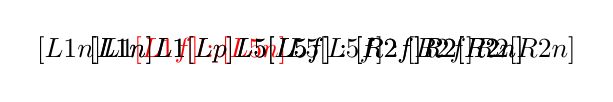
\begin{tikzpicture}
        \node<1> at(0,0){$[L1n]L1{\color{red}[L1f]:[L5n]}L5[L5f]:[R2f]R2[R2n]$};
        \node<2> at(0,0){$[L1n]L1{\color{red}[Lp]}L5[L5f]:[R2f]R2[R2n]$};
        \node<3> at(0,0){$[L1n]L1[Lp]L5[L5f]:[R2f]R2[R2n]$};
    \end{tikzpicture}}
    \item Only the segment $[L5f]:[R2f]$ is intermediate\\
    $${\color{red}Lp}=L5n<L5f=R2f<R2<{\color{red}R5}$$
\end{itemize}
\begin{center}
\g[0.6]{figures/star-before}
\end{center}
\end{frame}

\begin{frame}{\name}
$L1:L5:R2\enspace\xmapsto{\overset\Longleftarrow{R5}(\overline{Lp})}\enspace???$\\
\vfill
\pause Found $[L5f]:[R2f]$ as an intermediate segment
\begin{itemize}
    \item\pause Insert crossings $x_1$ and $x_2$
    \note<4>[item]{under because our finger is going above}
    $$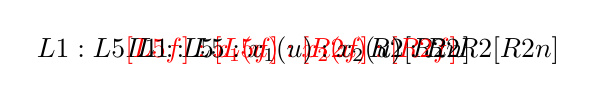
\begin{tikzpicture}
        \node<+> at(0,0){$L1:L5{\color{red}[L5f]:[R2f]}R2[R2n]$};
        \node<+> at(0,0){$L1:L5{\color{red}[L5f]:x_1(u):x_2(u):[R2f]}R2[R2n]$};
        \node<+-> at(0,0){$L1:L5:x_1(u):x_2(u):R2$};
    \end{tikzpicture}$$
\end{itemize}

\pause {Make spike for $R5$ and insert at $Lp$}

\begin{itemize}
    \item Spike: $x_2(o):R5:x_1(o)$
    $$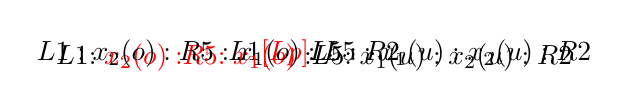
\begin{tikzpicture}
        \node<+> at(0,0){$L1{\color{red}[Lp]}L5:R2$};
        \node<+> at(0,0){$\stackrel\curvearrowright{L1}:{\color{red}x_2(o):\stackrel\curvearrowleft{R5}:x_1(o)}:\stackrel\curvearrowright{L5}:x_1(u):x_2(u):R2$};
        \node<+-> at(0,0){$L1:x_2(o):R5:x_1(o):L5:x_1(u):x_2(u):R2$};
    \end{tikzpicture}$$
\end{itemize}

\pause {Make twist on $R5$ (towards)}
$$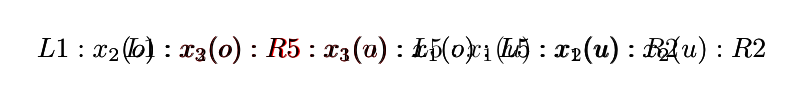
\begin{tikzpicture}
    \node<+> at(0,0){$L1:x_2(o):{\color{red}R5}:x_1(o):L5:x_1(u):x_2(u):R2$};
    \node<+> at(0,0){$L1:x_2(o):{\color{red}x_3(o):R5:x_3(u)}:x_1(o):L5:x_1(u):x_2(u):R2$};
    \node<+> at(0,0){$L1:x_2(o):{x_3(o):R5:x_3(u)}:x_1(o):L5:x_1(u):x_2(u):R2$};
\end{tikzpicture}$$
\end{frame}

\begin{frame}{\name}
$$\scriptstyle
L1:L5:R2\enspace\xmapsto{\overset\Longleftarrow{R5}(\overline{Lp})}\enspace L1:x_2(o):{x_3(o):R5:x_3(u)}:x_1(o):L5:x_1(u):x_2(u):R2
$$

\begin{center}
\g[0.4]{figures/star-before}$\xmapsto{\overset\Longleftarrow{R5}(\overline{Lp})}$
\g[0.4]{figures/star-pick-twist}
\end{center}
\end{frame}